\chapter{TZUNAMI PRE-MIGRATION ANALYZER FOR ECM SYSTEM}
This chapter gives an overview of \appName for different ECM systems. It contains the following topics.
\begin{itemize}
  \item Introduction
  \item Supported Systems for Analysis
  \item Key Features
  \item Licensing Information
\end{itemize}
 \section{INTRODUCTION}
 Tzunami Pre-migration is an application that scans the contents of the different ECM systems and generates reports. It helps the user to identify the possible hurdles and errors so that they can make the necessary changes or fixes on their source documents before the SharePoint migration. With the help of this feature, Truncate and Illegal Character map, available in the system we can suggest the user to make the necessary changes in their source document. User can also load the generated report by making the Spec file to the exporter.
 \\
So, \appName enables us to identify possible bottlenecks in the migration process beforehand. This will help to cut delays and re-work during migration process. The generated reports give us insight into the system and get us pre informed which helps to keep in track with our migration goal and business plan.
 \\
This guide provides detailed information about how to use \appName to a user.
\subsection{SUPPORTED SYSTEMS FOR ANALYSIS}
\appName supports following ECM systems:
 \\
ECM Systems:
 \\
\begin{enumerate}
  \item Atlassian Confluence
  \item EMC Documentum
  \item OpenText Livelink
  \item Xerox DocuShare
  \item OpenText Content Server
\end{enumerate}
\subsection{KEY FEATURES}
Following are some of the features of \appName:
\\
\begin{enumerate}
  \item Generates detail reports like size, total documents, files, folders, illegal files, long URL and unsupported extension based on selection made. Selection can be whole ECM or a portion of it.
  \item Displays metadata of each item.
  \item Displays security of each item.
  \item Option for exporting result in CSV format.
  \item Gives information about property set.
  \item Preview truncation of long file name, folder etc.
  \item Analyze ECM using filter condition.
  \item Gives graphical view of analyzed content.
\end{enumerate}
\subsection{LICENSING INFORMATION}
Tzunami Inc provides the license when you request for the license. Tzunami Inc sends login credential for license in email. You have to provide the credential in \appName. Once, you have got the license credential, perform following steps:
\\
\begin{enumerate}
\item	Open the \appName.
\item	Click on LicenseInfo in left bottom corner of the window.
\item	In the Update License window, provide the username and password, then click on Save button.
\item	You can view the license details by clicking on License Details button.
\end{enumerate}


\begin{figure} 
  \centering
	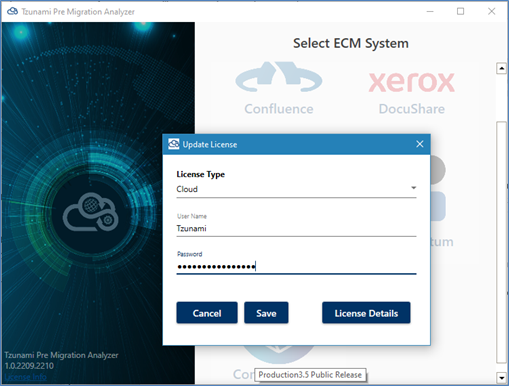
\includegraphics[width=0.8\textwidth]{Images/SelectEcmImage.png}
 \caption{Pre--migration Analyzer License}
\end{figure}
Tzunami Inc may provide the evaluation or full license based on your requirement. The evaluation license has the limitation of 10 items per folder analysis for all feature.
The \appName needs to communicate with Tzunami licensing server. Please, contact with your network administrator if there are any limitation, restriction or proxy environments and contact with Tzunami Support team. \\\\
If you cannot provide connection to Tzunami licensing server, please contact with Tzunami Support team at \href{mailto: sales@tzunami.com}{sales@tzunami.com} and inform with details. Tzunami Support team will contact back to you.
